%%%%%%%%%%%%%%%%%%%%%%%%%%%%%%%%%%%%%%%%%%%%%%%%%%%%%%%%%%%%%%%%%%% 
%                                                                 %
%                            CHAPTER FOUR                          %
%                                                                 %
%%%%%%%%%%%%%%%%%%%%%%%%%%%%%%%%%%%%%%%%%%%%%%%%%%%%%%%%%%%%%%%%%%% 

% EXPERIMENT COMMANDS
% ibeis -e rank_cdf --db humpbacks_fb -a default:has_any=hasnotch,mingt=2 -t default:proot=BC_DTW,decision=max,crop_dim_size=750,crop_enabled=True,manual_extract=True,use_te_scorer=True,ignore_notch=False,te_net=annot_res,te_score_method=avg,equalize_hist=False,kp_net=256_decoupled,tol=10 --dpath=/home/zach/data/results --save=<etc>.png --clipwhite

\chapter{Results} \label{sec:results}

In this chapter we present the results that our primary method achieves on the Flukebook dataset.
The main results for the optimal method are given briefly, and then we discuss how different variations on the method affect accuracy.

\section{Main method}

The main method we settled on achieves an 80\% top-1 accuracy on the dataset that we evaluated.  
The figures that we show in this section give the accuracy up to top-5 cumulatively.
In general we find that there are no surprises up to top-5, and that relative accuracies do not change significantly as we increase the rank at which we allow a match.
\\\\
The optimal configuration that we used for this method is given below.
\begin{itemize}
\item Crop size: 750px in width
\item We do not use the notch for trailing edge extraction
\item We set $n$ to $1$
\item We use the Residual architecture for scoring trailing edge
\item $\beta$ is set to $0.5$
\item We use [2\%, 4\%, 6\%, 8\%] for our curvature scales
\item We weight all curvature scales equally
\end{itemize}



\subsection{Characterization of Success cases}

Success and failure cases are difficult to characterize due to the nature of our dataset.  (TODO put in something real for this)

\subsection{Characterization of Failure cases}

Success and failure cases are difficult to characterize due to the nature of our dataset.  (TODO put in something real for this)

\section{Variations}

\subsection{Keypoint Extraction}

\subsubsection{Manual versus Automatic}


\begin{figure*}[t]%
\centering
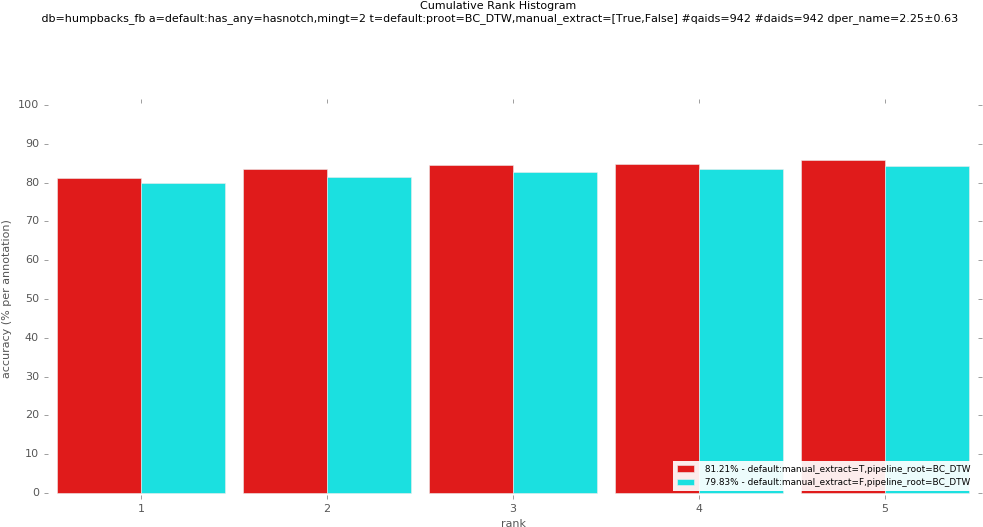
\includegraphics[width=1\textwidth]{../images/results/vary_manual_extract.png}
\caption[]{\textbf{Varying Manual Extraction}. We can see here that the difference in using the manually annotated points (purple) provided for this dataset versus the keypoint extractor's predicted points (cyan) produces a small drop in top-1 matching accuracy.}
\label{fig:vary_manual_extract}
\end{figure*}

One interesting note is to see how the final keypoint extractor compares with the manual annotations provided for the dataset.
We can see in Figure \ref{fig:manual_extract} that the manual extraction is only slightly better than the keypoint network extraction.
It is worth noting that none of the images in the keypoint network's training, validation, or even testing set came from the images evaluated here, so we believe that the keypoint extractor is very close to perfect for this task.
While this does not mean that the keypoints predicted are perfect, it does imply that they are ``good enough'' to extract a matchable trailing edge.

However, using the notch as the control point actually does reduce the accuracy more significantly for the predicted points than it does for the manually extracted points, which further implies that its predictions are not perfect.

\subsubsection{Varying training image sizes}

Intuitively, the bigger the image the better the prediction can be, but at the expense of requiring more parameters to handle the input.
The primary difference between the networks that were trained to handle different size inputs is that, in order to ensure that all inputs to the final dense layers have the same spatial size ($2\times2$) across the different networks, an extra convolutional and pooling layer is added.

The performance of networks trained and run on different sized images is given in Figure \ref{fig:vary_kp_size}.

\begin{figure*}[t]%
\centering
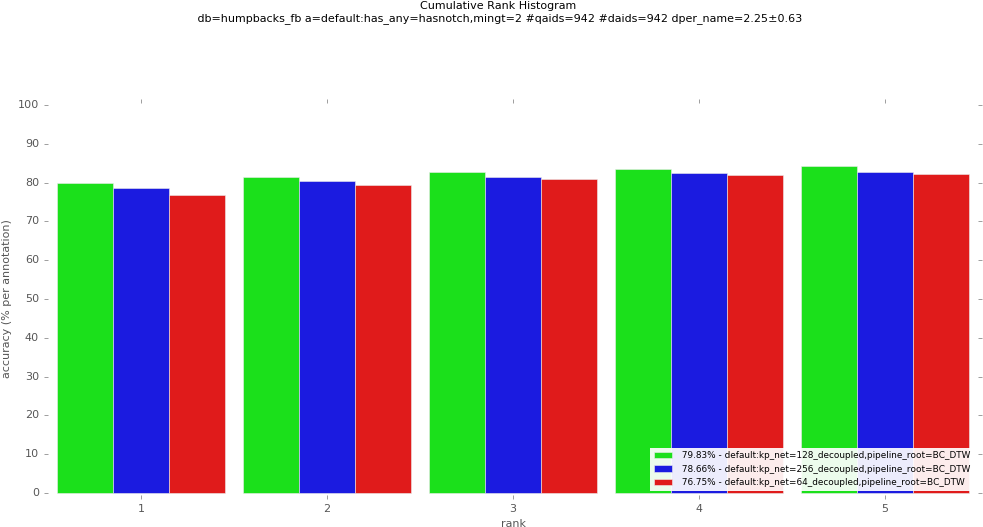
\includegraphics[width=1\textwidth]{../images/results/vary_kp_size.png}
\caption[]{\textbf{Varying Keypoint Image Size}. While the $128 \times 128$ size network is better than the $256 \times 256$ network (green and blue respectively), we believe the difference between them to be insignificant. The $644 \times 64$ network (red) is clearly inferior however. }
\label{fig:vary_kp_size}
\end{figure*}


We trained each of these networks on separate splits of data, and due to the inherent stochasticity of the training it is difficult to ascertain whether or not the image size is a cause of performance issues. 


\subsubsection{STN} % Maybe?

We also briefly experimented with an Spatial Transformer Network.
This was largely motivated by the tendency of the keypoint extractor to do a terrible job of predicting fluke keypoints on flukes that did not 'fill' the image horizontally.
Unfortunately, we could not get the STN to converge at a better accuracy than the standard keypoint extractor, even if we held its parameters fixed for a few training epochs.
Usually, the STN would produce nonsensical transformations of the image.

% TODO: Figure showing this

\subsection{Image Preprocessing}

In this part we also detail some simple image preprocessing steps that we took (given the fluke keypoints) that greatly influenced the efficacy of the method.
Ultimately we just ended up using a combination of cropping and resizing the image so as to normalize the length of the trailing edge, as detailed below.

We also note that we originally tried histogram equalization as part of the preprocessing pipeline, althoough it produced significantly worse trailing edges (and subsequently matching accuracy).

\subsubsection{Cropping and Image Width}

While, with dynamic time warping, we theoretically can match sequences of similar or different lengths, the distances are distorted by large differences in actual trailing edge length.
Since we are only interested in the width of an image (assuming that the trailing edge is roughly horizontal in the image), we can get every trailing edge to have exactly some fixed length $w$ by the following process

\begin{itemize}
    \item Crop the image horizontally between the left and right columns found by the keypoint extraction process (or manually determined).
    \item Resize the cropped image to some fixed width $w$ while preserving the aspect ratio, using Lanczos interpolation. % Maybe find citation for this
\end{itemize}

In this way, we standardize the trailing edge length so that image scale does not affect detection accuracy too much.

One major caveat with this process is of course that using the keypoint extractor's predictions can cause catastrophic failures in this process (e.g. the left and right points are nowhere near a fluke), however in practice we found that it works well enough -- far better than the alternative.

We can see in Figure \ref{fig:vary_crop_nocrop} that cropping and resizing is absolutely vital to the performance of our algorithm.

\begin{figure*}[t]%
\centering
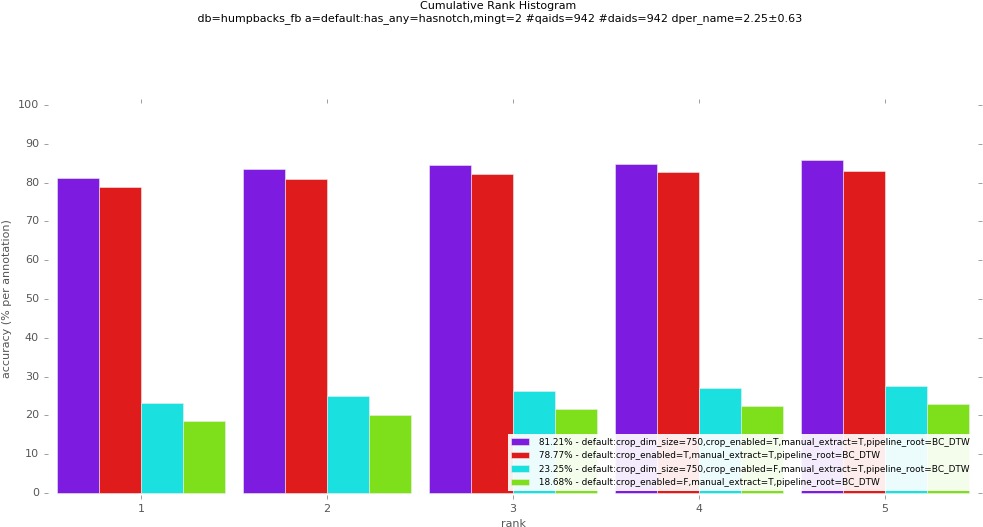
\includegraphics[width=1\textwidth]{../images/results/vary_crop_nocrop.png}
\caption[]{\textbf{Varying Crop Strategy}. Cropping images around the trailing edge and then resizing them proves to be very important, not doing so gives a very low accuracy. We can see in Figure \ref{fig:chip_size_hist} that there is a wide distribution of image sizes, which can hamper the effectiveness of DTW.}
\label{fig:vary_crop_nocrop}
\end{figure*}

\begin{figure*}[t]%
\centering
\subfloat[Distribution of Image Widths][]{
	\includegraphics[width=0.5\textwidth]{../images/results/chip_width_hist_fb.png}
}
\subfloat[Distribution of Trailing Edge Lengths][]{
	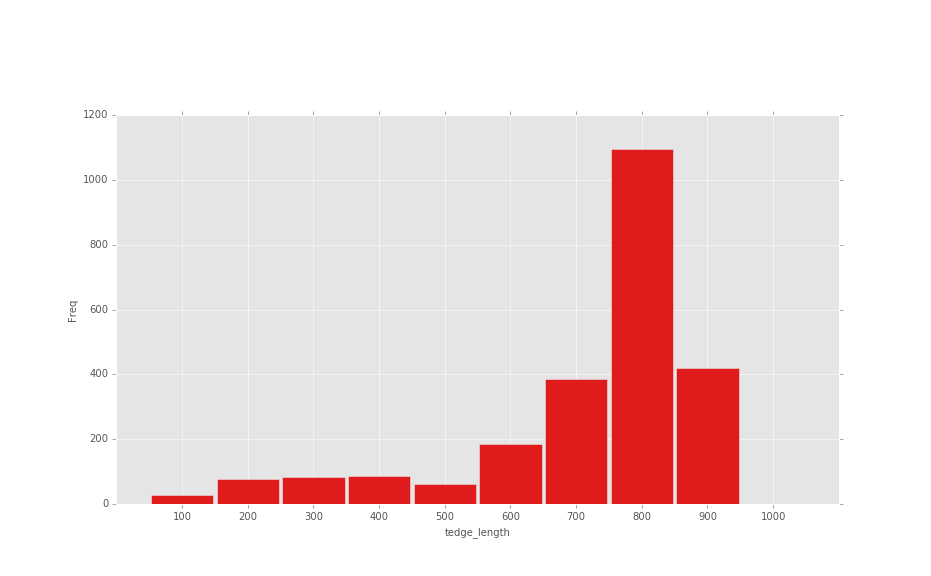
\includegraphics[width=0.5\textwidth]{../images/results/te_size_hist_fb.png}
}
\caption[]{\textbf{Distribution of Image Widths}. The image width distribution (left) is fairly wide, with most of the mass centered between 600 and 800.}
\label{fig:width_te_dist}
\end{figure*}



\paragraph{Trailing Edge Length}

Determining what $w$ should be is not super obvious.
Ideally, one would simply look at the mode or average post-crop width, and try to keep $w$ around there, since intuitively we want to introduce as few interpolation artifacts from resizing as possible.

We can see in Figure \ref{fig:vary_crop_size} that the optimal post-crop $w$ for this dataset (of the few we evaluated) is 750 pixels, althout 1000 pixels is on par.
We select the former for efficiency's sake, as smaller trailing edges vastly improves the speed of the matching algorithm.
Figure \ref{fig:width_te_dist:b} shows the histogram of post-crop widths (i.e\ trailing edge lengths), showing a large concentration of mass around 800 pixels 
This confirms that the less the image has to be resized, the better the trailing edge.

\begin{figure*}[t]%
\centering
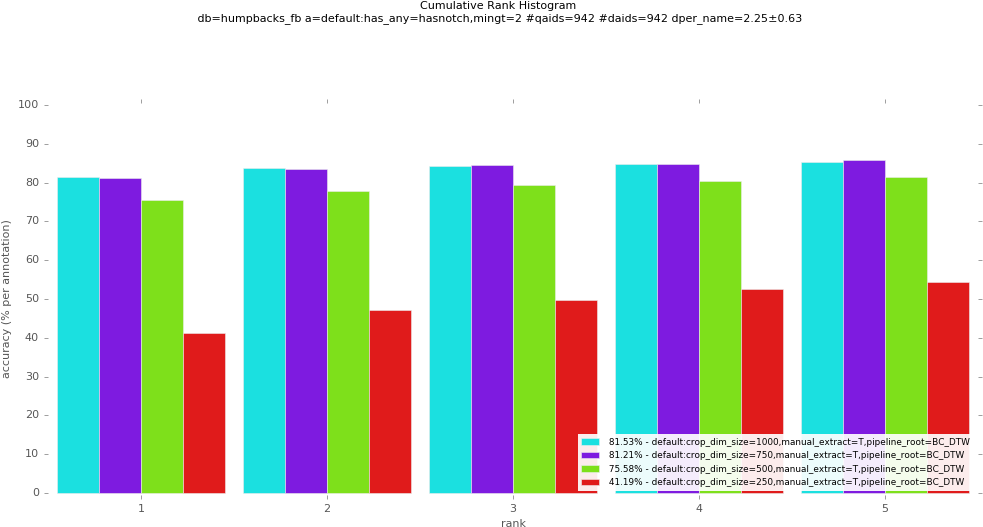
\includegraphics[width=1\textwidth]{../images/results/vary_crop_size.png}
\caption[]{\textbf{Varying Crop Size}. Since we crop around the start and end points of the trailing edge, this crop size effectively controls the length of the extracted trailing edge. Note that we use the manually annotated points in this analysis to control for any issues with keypoint extraction.}
\label{fig:vary_crop_size}
\end{figure*}


\subsection{Trailing Edge Extraction}

One major result that we found was that, when using the averaging method to combine the trailing edge scores with $N_y$, having a robust trailing edge prediction wasn't as important as having a detailed trailing edge.


\subsubsection{Trailing Edge Scorer variations}

The various trailing edge scorer architectures and their results on the task they were trained for is detailed in the previous chapter.
In Figure \ref{fig:vary_te_scorer} we present the actual matching accuracies that each one produced.

We can see that the detailed and higher quality trailing edges produced by the Residual network give a decent performance boost over the other networks.
The only other network that beats not using the trailing edge scorer at all (i.e.\ $\beta = 0$, see the purple bar in Figure \ref{fig:vary_te_weight}) is the Simple network.

We hypothesize that the Jet and Upsample architectures do poorly due to their inability to produce fine-grained trailing edges. % TODO: look at discrepancies to verify this

\begin{figure*}[t]%
\centering
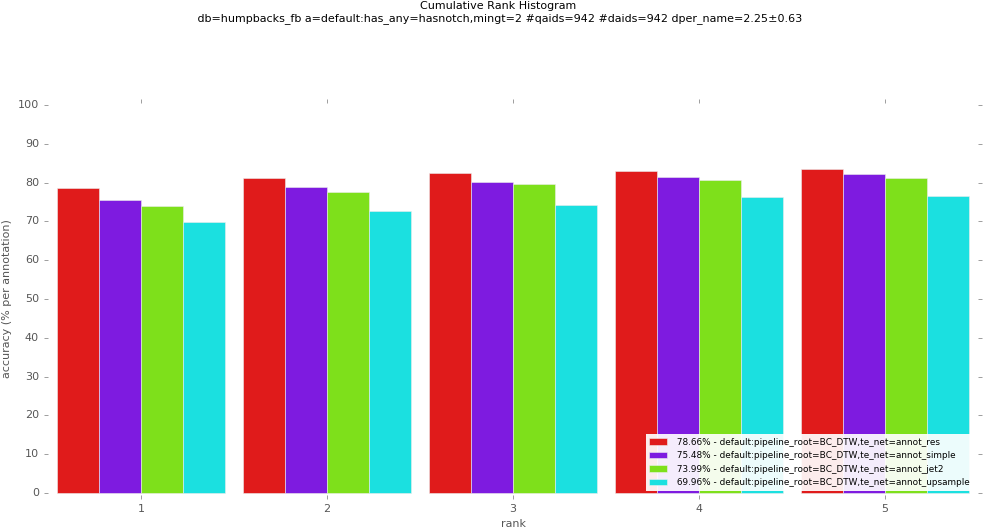
\includegraphics[width=1\textwidth]{../images/results/vary_te_scorer.png}
\caption[]{\textbf{Trailing Edge Scorer Architectures}. The highest performing trailing edge scorer (Residual) is shown in red, followed by Simple, Jet, and Upsample (in descending order of accuracy).}
\label{fig:vary_te_scorer}
\end{figure*}

One caveat with using the Residual network is that, with 64 layers, it consumes a lot of GPU memory.

\subsubsection{Combining $N_y$ and $T_y$}

We only evaluate the 'average' method here, and show that the mixing parameter $\beta$ has a significant effect on matching accuracy.

In Figure \ref{fig:vary_te_weight}, we can see that simply a pixel-wise average of $N_y$ and $(1-T_y)$ (i.e. $\beta = 0.5$) produces the best results for the Residual network.

\begin{figure*}[t]%
\centering
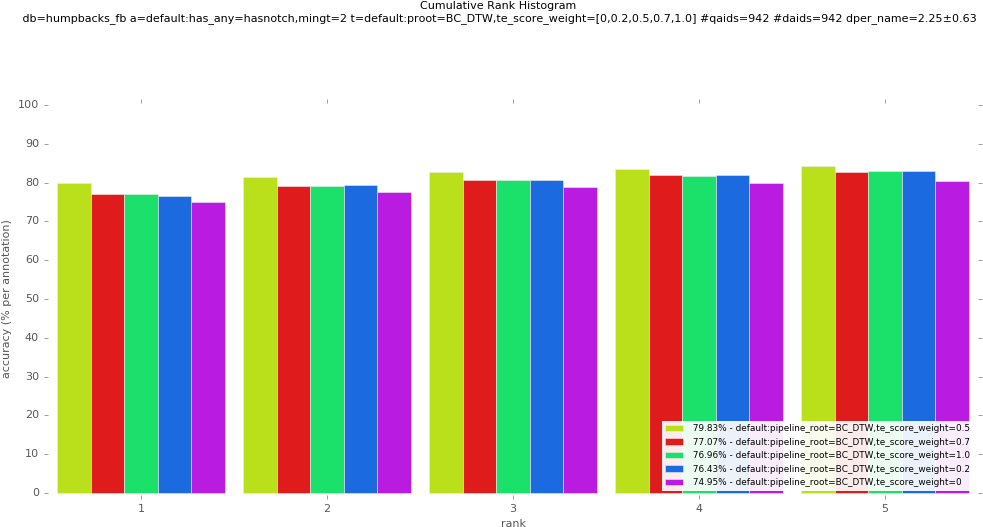
\includegraphics[width=1\textwidth]{../images/results/vary_te_weight.png}
\caption[]{\textbf{Varying $\beta$}. It's clear from this that the optimal $\beta$ is $0.5$, although it is interesting to note that using only the network's trailing edge scores provides better accuracy than not using it at all.}
\label{fig:vary_te_weight}
\end{figure*}


\subsubsection{Number of neighbors in the extraction}

The number of neighbors $n$ effectively limits the slope of the trailing edge.
We limit it to an odd number for convenience.
On the one hand, a lower $n$ can cause the trailing edge to be limited in vertical breadth, but does prevent it from going way off course.
Despite this, with trailing edge scoring in place, it might be beneficial to increase $n$ so as to avoid parts of the trailing edge that continually ``max out'' the number of neighbors.

Ultimately, we can see in Figure \ref{fig:vary_neighbors} that limiting the number of neighbors to the immediate neighborhood (i.e. $n = 3$) produces a significant boost over a larger neighborhood.
While the trailing edges extracted with $n = 3$ can be somewhat less detailed, they are less likely to go completely off course.
Additionally, despite the trailing edges being less detailed, the extraction artifacts (i.e.\ the parts of the trailing edge that ``max out'') are produced in a way that is unique to the trailing edge, which may explain the accuracy boost.

\begin{figure*}[t]%
\centering
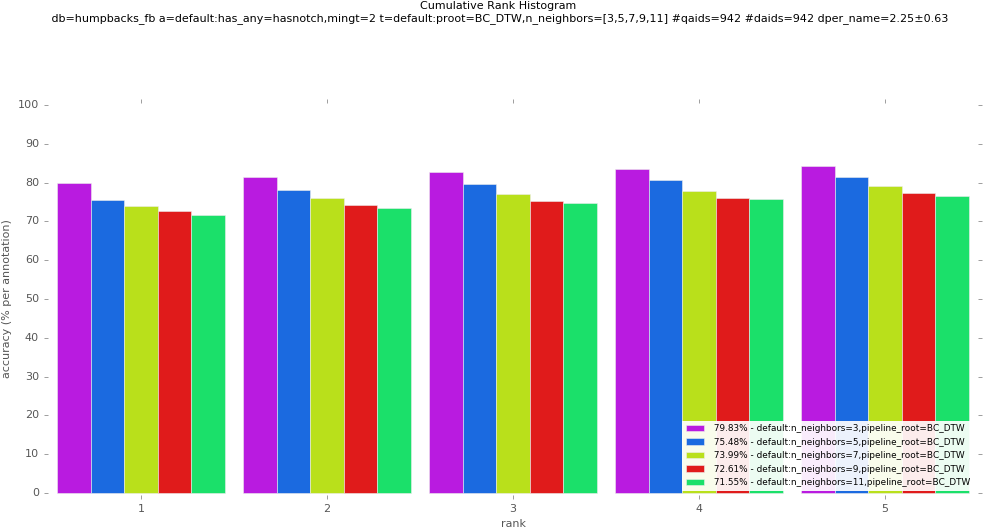
\includegraphics[width=1\textwidth]{../images/results/vary_neighbors.png}
\caption[]{\textbf{Varying $n$}. This shows that the optimal neighborhood constraint is $n = 1$, despite qualitatively producing worse-looking trailing edges.}
\label{fig:vary_neighbors}
\end{figure*}



\subsection{Curvature Extraction}

Curvature extraction is one of the least parameterized part of the process, however figuring out what the optimal scales to extract are and how many is non-trivial.
One major point is that increasing the cardinality of $S$ increases the time it takes to evaluate the dynamic time warping, and as such we try to keep it at a small value (i.e. $|S| = 4$).

\subsubsection{Different scales}

We can look at each scale as measuring the curvature of some percentage of the trailing edge around the given point.
Intuitively, since the meaningful differences in trailing edge can be fairly small, it makes sense to measure a small curvature scale.
Additionally, this gives the most diversity in the trailing edge, as larger curvatures will change less and less from one point to the next.

However, larger curvatures are also less sensitive to noise, and thus small trailing edge extraction failures.


\begin{figure*}[t]%
	\centering
	\subfloat[][]{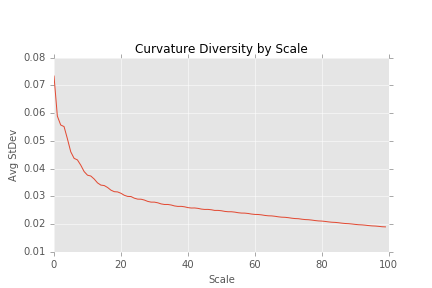
\includegraphics[width=0.5\textwidth]{../images/results/curvature_diversity_fb.png} }%
	\subfloat[][]{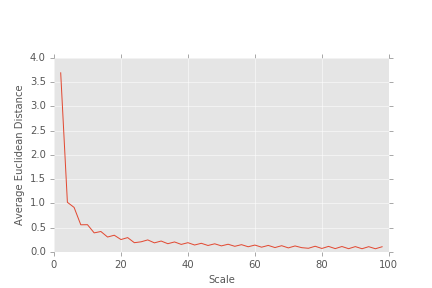
\includegraphics[width=0.5\textwidth]{../images/results/interscale_diff_fb.png} }%
	\caption[]{\textbf{Curvature Diversity}. Left panel (a) shows the average standard deviation of the (fixed length) curvature at different scales. Right panel (b) shows the average Euclidean distance between successive scales of curvature}
    	\label{fig:curvature_diversity}
\end{figure*}


We find that (as shown in the left panel of Figure \ref{fig:curvature_diversity}) as block curvature scale is increased, the diversity at any given point in the curvature (if it is of a fixed size) goes down drastically. 
As a result, we stick to the lower end of the scale, keeping the curvature scales measured below 15\%.

We can also see on the right side of Figure \ref{fig:curvature_diversity} that successive curvature scales show bigger differences at lower scales than at higher scales, which reinforces this need, but that it's advantageous to make bigger jumps between scales to maximize diversity while minimizing computation time.

Based on the above, we evaluate scales that run from 1\% to 10\%, with varying levels of resolution.
Overall we found that this does not have a major effect on accuracy, but that the scales [2\%, 4\%, 6\%, 8\%] provides marginally better accuracy than anything else that we tried.
This is shown in Figure \ref{vary_curv_scales}

\begin{figure*}[t]%
\centering
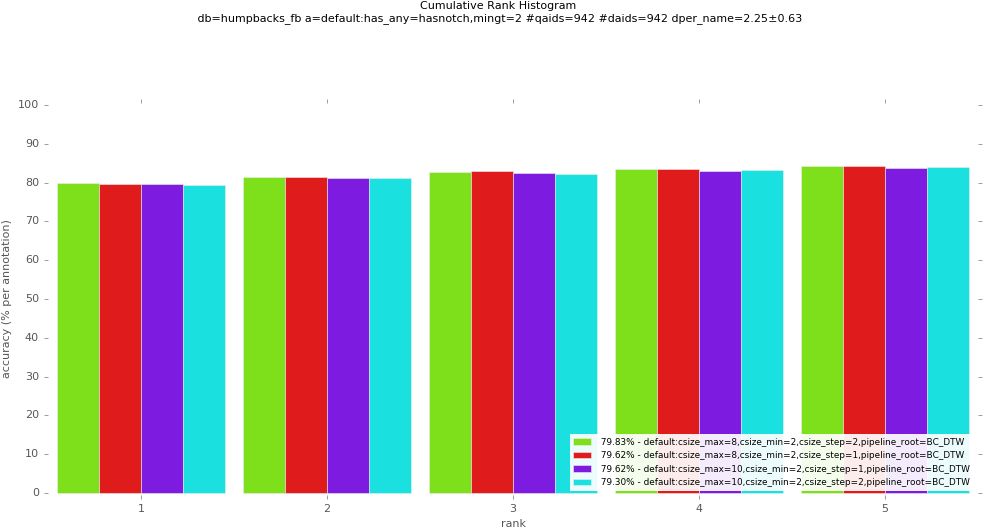
\includegraphics[width=1\textwidth]{../images/results/vary_curv_scales.png}
\caption[]{\textbf{Varying Curvature Scales}. The scales evaluated here are parameterized with a start, end, and step size. We always start at 2\%, and vary the step size between 1 \& 2 and the end between 8\% \& 10\%.}
\label{fig:vary_curv_scales}
\end{figure*}

\subsection{Dynamic Time Warp Matching}

The main variants shown in this section are the different Sakoe-Chiba bound windows and the scale weighting term in the curvature distance function.

\subsubsection{Weighting the different scales}

There are many ways to produce the weights $s_w$ for curvatures, but intuitively there should be a monotonic relationship between curvature scale and importance.

We could specify this relationship as a ratio $W$ of importance between successive pairs of curvatures (increasing in size).
We parameterize that importance by giving each scale the weight $s_w = [W^i \forall i \in [0,|S|]$.
In order to maintain this ratio without blowing up the distances, we also normalize so that $\sum s_w = 1$.

\begin{figure*}[t]%
\centering
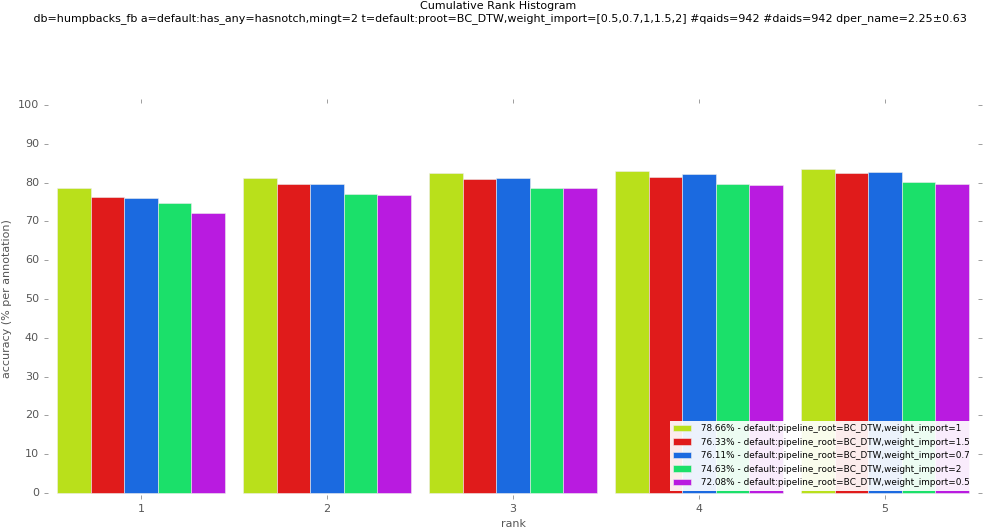
\includegraphics[width=1\textwidth]{../images/results/vary_weight_import.png}
\caption[]{\textbf{Varying $s_w$}. The yellow bar shows $W = 1$, i.e.\ all curvatures weighted equally.}
\label{fig:vary_weight_import}
\end{figure*}



Figure \ref{fig:vary_weight_import} shows that despite this effort, it appears that equally weighting each curvature scale provides the best performance.
Interestingly weighting larger scales lower (i.e.\ $W < 1$, which we evaluate with $W = 0.5$ (purple bar) in Figure \ref{fig:vary_weight_import}) provides worse performance.

\subsubsection{Window size}

In Figure \ref{fig:vary_window}, we can see that if we decrease the window (i.e. the Sakoe-Chiba bound) size, at around 10\% of the query trailing edge length we maintain the same accuracy as the full window (i.e. 100\%), but below this accuracy is severely affected.
We find that overall there is a $4\times$ slow-down in wall-clock time on our testing machine when going from a window size of 10\% to one of 100\%. 
Thus, we use this value for the window size so as to minimize computation time while maintaining the total accuracy.

Additionally, while it's possible for gross mismatches to occur from there being no window boundary, we can see from Figure \ref{fig:vary_window} that this does not pose a problem in our case.

\begin{figure*}[t]%
\centering
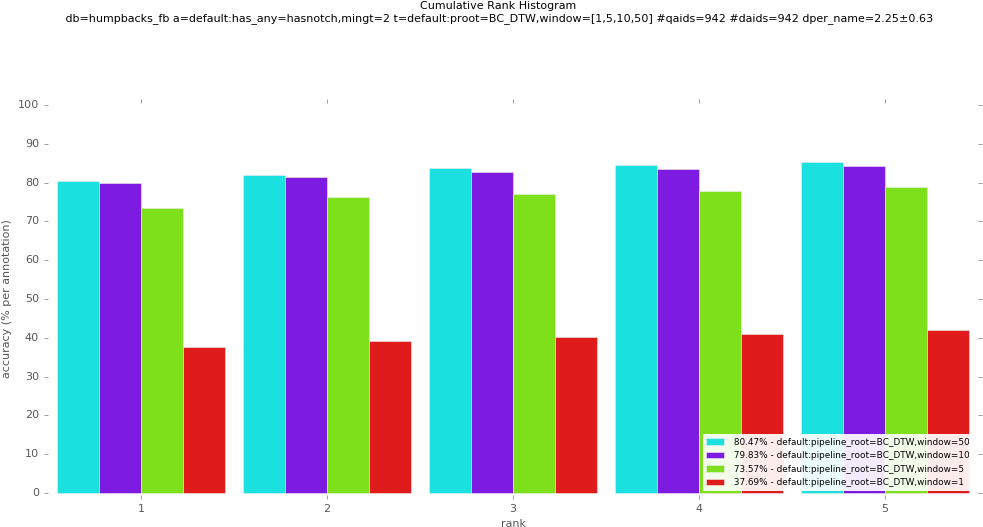
\includegraphics[width=1\textwidth]{../images/results/vary_window.png}
\caption[]{\textbf{Varying Sakoe-Chiba bound}}
\label{fig:vary_window}
\end{figure*}

\subsubsection{Aggregating over multiple trailing edges per identity}

Determining the identity of a given query image given distances to other images in the database is not entirely simple when there are multiple database images for a given individual.
Essentially we need to transform these distances from query image to database image into distances from query to known individual.
To do so we evaluate two options given a group of distances for an individual --- either the average distance or the minimum distance.

We find that the average decision does slightly better, as shown in Figure \ref{fig:vary_decision}.

This is unsurprising given that most of the individuals in the dataset only have two images associated, meaning that the average is equivalent to the minimum.
That said, the minimal distance criterion is effectively the single-feature case of LNBNN used in Hotspotter \cite{crall_hotspotter_2013} and the work of Hughes et al.\ \cite{hughes2015automated}. % TODO: lay out what this theoretical backing actually is

\begin{figure*}[t]%
\centering
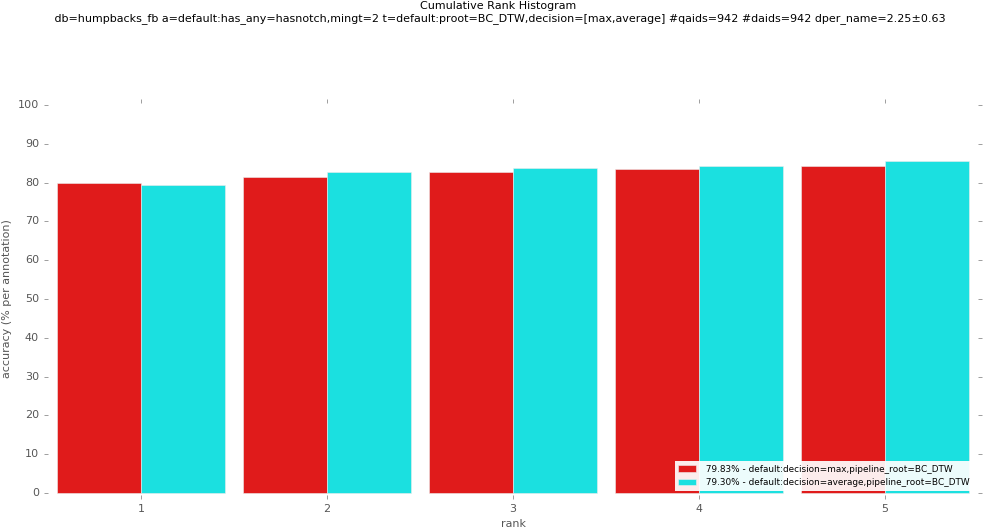
\includegraphics[width=1\textwidth]{../images/results/vary_decision.png}
\caption[]{\textbf{Varying Decision Criterion}}
\label{fig:vary_decision}
\end{figure*}

\section{In Combination with Hotspotter}

By combining our method with Hotspotter --- if we were able to automatically pick out which algorithm was right for a given ranking --- we can achieve 93\% accuracy on the Flukebook dataset.

(TODO: this)

\subsection{Failure cases}

(TODO: this)

\subsection{Characterization of when to use which method}

From an intuitive standpoint, it appears that Hotspotter cannot find effective keypoints from trailing edges, which hampers its ability to handle flukes which do not have an apparent pattern.

We hypothesize that this is because the trailing edge --- while a distinctive feature --- inevitably shares a region with an oceanic background.
Since this oceanic background changes from image to image, it cannot find meaningful matches.

(TODO: this)

%%% Local Variables: 
%%% mode: latex
%%% TeX-master: t
%%% End: 
